\chapter{Objects and morphisms}
\label{ch:cats}
I can't possibly hope to do category theory any justice in these few chapters;
thus I'll just give a very high-level overview of how many of the concepts we've
encountered so far can be re-cast into categorical terms.
So I'll say what a category is, give some examples,
then talk about a few things that categories can do.
For my examples, I'll be drawing from all the previous chapters;
feel free to skip over the examples corresponding to things you haven't seen.

If you're interested in category theory (like I was!), perhaps in
what surprising results are true for general categories, I strongly recommend \cite{ref:msci}.

\section{Motivation: isomorphisms}
From earlier chapters let's recall the definition of an \emph{isomorphism} of two objects:
\begin{itemize}
	\ii Two groups $G$ and $H$ are isomorphic if there was a bijective homomorphism:
	equivalently, we wanted homomorphisms $\phi : G \to H$ and $\psi : H \to G$
	which were mutual inverses, meaning $\phi \circ \psi = \id_H$ and $\psi \circ \phi = \id_G$.
	\ii Two metric (or topological) spaces $X$ and $Y$ are isomorphic
	if there is a continuous bijection $f : X \to Y$ such that $f\inv$ is also continuous.
	\ii Two vector spaces $V$ and $W$ are isomorphic if there is a bijection $T : V \to W$
	which is a linear map.
	Again, this can be re-cast as saying that $T$ and $T\inv$ are linear maps.
	\ii Two rings $R$ and $S$ are isomorphic if there is a bijective ring homomorphism $\phi$;
	again, we can re-cast this as two mutually inverse ring homomorphisms.
\end{itemize}

In each case we have some collections of objects and some maps,
and the isomorphisms can be viewed as just maps.
Let's use this to motivate the definition of a general \emph{category}.

\section{Categories, and examples thereof}
\prototype{$\catname{Grp}$ is possibly the most natural example.}
\begin{definition}
	A \vocab{category} $\AA$ consists of:
	\begin{itemize}
		\ii A class of \vocab{objects}, denoted $\obj(\AA)$.
		\ii For any two objects $A_1, A_2 \in \obj(\AA)$, 
		a class of \vocab{arrows} (also called \vocab{morphisms} or \vocab{maps}) between them.
		We'll denote the set of these arrows by $\Hom_\AA(A_1, A_2)$.
		\ii For any $A_1, A_2, A_3 \in \obj(\AA)$,
		if $f \colon A_1 \to A_2$ is an arrow and $g \colon A_2 \to A_3$ is an arrow,
		we can compose these arrows to get an arrow $g \circ f \colon A_1 \to A_3$.

		We can represent this in a \vocab{commutative diagram}
		\begin{center}
		\begin{tikzcd}
			A_1 \ar[r, "f"] \ar[rd, "h"'] & A_2 \ar[d, "g"] \\
			& A_3
		\end{tikzcd}
		\end{center}
		where $h = g \circ f$.
		The composition operation $\circ$ is part of the data of $\AA$;
		it must be associative.
		In the diagram above we say that $h$ \vocab{factors} through $A_2$.
		
		\ii Finally, every object $A \in \obj(\AA)$ has a special \vocab{identity arrow} $\id_A$;
		you can guess what it does.\footnote{To be painfully explicit:
			if $f \colon A' \to A$ is an arrow then $\id_A \circ f = f$;
		similarly, if $g \colon A \to A'$ is an arrow then $g \circ \id_A = g$.}
	\end{itemize}
\end{definition}
\begin{abuse}
	From now on, by $A \in \AA$ we'll mean $A \in \obj(\AA)$.
\end{abuse}
\begin{abuse}
	You can think of ``class'' as just ``set''.
	The reason we can't use the word ``set'' is
	because of some paradoxical issues with
	collections which are too large;
	Cantor's Paradox says there is no set of all sets.
	So referring to these by ``class'' is a way of sidestepping these issues.

	Now and forever I'll be sloppy and assume all my categories
	are \vocab{locally small}, meaning that $\Hom_{\AA} (A_1, A_2)$
	is a set for any $A_1, A_2 \in \AA$.
	So elements of $\AA$ may not form a set,
	but the set of morphisms between
	two \emph{given} objects will always assumed to be a set.
\end{abuse}

Let's formalize the motivation we began with.
\begin{example}
	[Basic examples of categories]
	\listhack
	\label{example:basic_categories}
	\begin{enumerate}[(a)]
		\ii There is a category of groups $\catname{Grp}$. The data is
		\begin{itemize}
			\ii The objects of $\catname{Grp}$ are the groups.
			\ii The arrows of $\catname{Grp}$ are the homomorphisms between these groups.
			\ii The composition $\circ$ in $\catname{Grp}$ is function composition.
		\end{itemize}
		\ii In the same way we can conceive a category $\catname{CRing}$ of (commutative) rings.
		\ii Similarly, there is a category $\catname{Top}$ of topological spaces,
		whose arrows are the continuous maps.
		\ii There is a category $\catname{Top}_\ast$ of topological spaces with a \emph{distinguished basepoint};
		that is, a pair $(X, x_0)$ where $x_0 \in X$.
		Arrows are continuous maps $f : X \to Y$ with $f(x_0) = y_0$.
		\ii Similarly, there is a category $\catname{Vect}_k$ of
		vector spaces (possibly infinite-dimensional) over a field $k$,
		whose arrows are the linear maps.
		There is even a category $\catname{FDVect}_k$ of
		\emph{finite-dimensional} vector spaces.
		\ii We have a category $\catname{Set}$ of sets,
		where the arrows are \emph{any} maps.
	\end{enumerate}
\end{example}
And of course, we can now define what an isomorphism is!
\begin{definition}
	An arrow $A_1 \taking{f} A_2$ is an \vocab{isomorphism}
	if there exists $A_2 \taking{g} A_1$ such that $f \circ g = \id_{A_2}$
	and $g \circ f = \id_{A_1}$.
	In that case we say $A_1$ and $A_2$ are \vocab{isomorphic}, hence $A_1 \cong A_2$.
\end{definition}
\begin{remark}
	Note that in $\catname{Set}$, $X \cong Y
	\iff \left\lvert X \right\rvert = \left\lvert Y \right\rvert$.
\end{remark}
\begin{ques}
	Check that every object in a category is isomorphic to itself.
	(This is offensively easy.)
\end{ques}
More importantly, this definition should strike you as a little impressive.
We're able to define whether two groups (rings, spaces, etc.) are isomorphic
solely by the functions between the objects.
Indeed, one of the key themes in category theory (and even algebra) is that
\begin{moral}
	One can learn about objects by the functions between them.
	Category theory takes this to the extreme by \emph{only} looking at arrows,
	and ignoring what the objects themselves are.
\end{moral}

But there are some trickier interesting examples of categories.
\begin{example}
	[Posets are categories]
	Let $\mathcal P$ be a partially ordered set.
	We can construct a category $P$ for it as follows:
	\begin{itemize}
		\ii The objects of $P$ are going to be the elements of $\mathcal P$.
		\ii The arrows of $P$ are defined as follows:
		\begin{itemize}
			\ii For every object $p \in P$, we add an identity arrow $\id_p$, and
			\ii For any pair of distinct objects $p \le q$, we add a single arrow $p \to q$.
		\end{itemize}
		There are no other arrows.
		\ii There's only one way to do the composition. What is it?
	\end{itemize}
\end{example}
For example, for the poset $\mathcal P$ on four objects $\{a,b,c,d\}$ with $a \le b$ and $a \le c \le d$, we get:
\begin{center}
\begin{tikzpicture}[scale=3.5]
	\SetVertexMath
	\Vertices{square}{d,c,a,b}
	\Edge[style={->}, label={$a \le b$}](a)(b)
	\Edge[style={->}, label={$a \le c$}](a)(c)
	\Edge[style={->}, label={$a \le d$}](a)(d)
	\Edge[style={->}, label={$c \le d$}](c)(d)
	\Loop[dist=8, dir=NO, label={$\id_a$}, labelstyle={above=1pt}](a)
	\Loop[dist=8, dir=WE, label={$\id_b$}, labelstyle={left=1pt}](b)
	\Loop[dist=8, dir=EA, label={$\id_c$}, labelstyle={right=1pt}](c)
	\Loop[dist=8, dir=WE, label={$\id_d$}, labelstyle={left=1pt}](d)
\end{tikzpicture}
\end{center}

This illustrates the point that
\begin{moral}
	The arrows of a category can be totally different from functions.
\end{moral}
In fact, in a way that can be made precise, the term ``concrete category'' refers
to one where the arrows really are ``structure-preserving maps between sets'',
like $\catname{Grp}$, $\catname{Top}$, or $\catname{CRing}$.

\begin{ques}
	Check that no two distinct objects of a poset are isomorphic.
\end{ques}

Here's a second quite important example of a non-concrete category.
\begin{example}
	[Important: groups are one-Object categories]
	A group $G$ can be interpreted as a category $\mathcal G$ with one object $\ast$,
	all of whose arrows are isomorphisms.

	\begin{center}
	\begin{tikzpicture}[scale=5.5]
		\Vertex[x=0,y=0,L={$\ast$}]{a}
		\Loop[dist=8, dir=NO, label={$1 = \id_a$}, labelstyle={above=1pt}](a)
		\Loop[dist=7, dir=WE, label={$g_2$}, labelstyle={left=1pt}](a)
		\Loop[dist=9, dir=SO, label={$g_3$}, labelstyle={below=1pt}](a)
		\Loop[dist=8, dir=EA, label={$g_4$}, labelstyle={right=1pt}](a)
	\end{tikzpicture}
	\end{center}

	As \cite{ref:msci} says:

	\begin{quote}
	The first time you meet the idea that a group is a kind of category,
	it's tempting to dismiss it as a coincidence or a trick.
	It's not: there's real content.
	To see this, suppose your education had been shuffled and you took a course
	on category theory before ever learning what a group was.
	Someone comes to you and says: 

	``There are these structures called `groups', and the idea is this:
	a group is what you get when you collect together all the symmetries
	of a given thing.''

	``What do you mean by a `symmetry'?'' you ask.

	``Well, a symmetry of an object $X$ is a way of transforming $X$ or mapping
	$X$ into itself, in an invertible way.''

	``Oh,'' you reply, ``that's a special case of an idea I've met before.
	A category is the structure formed by \emph{lots} of objects and mappings
	between them -- not necessarily invertible. A group's just the very special case
	where you've only got one object, and all the maps happen to be invertible.''
	\end{quote}
\end{example}

\begin{exercise}
	Verify the above!
	That is, show that the data of a one-object category with all isomorphisms
	is the same as the data of a group.
\end{exercise}

Finally, here are some examples of categories you can make from other categories.
\begin{example}
	[Deriving categories]
	\listhack
	\begin{enumerate}[(a)]
		\ii Given a category $\AA$, we can construct the \vocab{opposite category}
		$\AA\op$, which is the same as $\AA$ but with all arrows reversed.
		\ii Given categories $\AA$ and $\BB$, we can construct the \vocab{product category} $\AA \times \BB$
		as follows: the objects are pairs $(A, B)$ for $A \in \AA$ and $B \in \BB$,
		and the arrows from $(A_1, B_1)$ to $(A_2, B_2)$
		are pairs \[ \left( A_1 \taking{f} A_2, B_1 \taking{g} B_2 \right). \]
		What do you think the composition and identities are?
	\end{enumerate}
\end{example}

\section{Special objects in categories}
\prototype{$\catname{Set}$ has initial object $\varnothing$ and final object $\{\ast\}$. An element of $S$ corresponds to a map $\{\ast\} \to S$.}
Certain objects in categories have special properties.
Here are a couple examples.
\begin{example}
	[Initial object]
	An \vocab{initial object} of $\AA$ is an object
	$A_{\text{init}} \in \AA$ such that for any $A \in \AA$ (possibly $A = A_{\text{init}}$),
	there is exactly one arrow from $A_{\text{init}}$ to $A$.
	For example,
	\begin{enumerate}[(a)]
		\ii The initial object of $\catname{Set}$ is the empty set $\varnothing$.
		\ii The initial object of $\catname{Grp}$ is the trivial group $\{1\}$.
		\ii The initial object of $\catname{CRing}$ is the ring $\ZZ$
		(recall that ring homomorphisms $R \to S$ map $1_R$ to $1_S$).
		\ii The initial object of $\catname{Top}$ is the empty space.
		\ii The initial object of a partially ordered set is its smallest element, if one exists.
	\end{enumerate}
\end{example}

We will usually refer to ``the'' initial object of a category, since:
\begin{exercise}
	[Important!]
	Show that any two initial objects $A_1$, $A_2$ of $\AA$ are \emph{uniquely isomorphic}
	meaning there is a unique isomorphism between them.
\end{exercise}

\begin{remark}
	In mathematics, we usually neither know nor care if two objects are actually equal
	or whether they are isomorphic.
	For example, there are many competing ways to define $\RR$,
	but we still just refer to it as ``the'' real numbers.

	Thus when we define categorical notions, we would like to check they are
	unique up to isomorphism.
	This is really clean in the language of categories, and definitions
	often cause objects to be unique up to isomorphism for elegant reasons like the above.
\end{remark}

One can take the ``dual'' notion, a terminal object.
\begin{example}
	[Terminal object]
	A \vocab{terminal object} of $\AA$ is an object
	$A_{\text{final}} \in \AA$ such that for any $A \in \AA$ (possibly $A = A_{\text{final}}$),
	there is exactly one arrow from $A$ to $A_{\text{final}}$.
	For example,
	\begin{enumerate}[(a)]
		\ii The terminal object of $\catname{Set}$ is the singleton set $\{\ast\}$.
		(There are many singleton sets, of course, but \emph{as sets} they are all isomorphic!)
		\ii The terminal object of $\catname{Grp}$ is the trivial group $\{1\}$.
		\ii The terminal object of $\catname{CRing}$ is the zero ring $0$.
		(Recall that ring homomorphisms $R \to S$ must map $1_R$ to $1_S$).
		\ii The terminal object of $\catname{Top}$ is the single-point space.
		\ii The terminal object of a partially ordered set is its maximal element, if one exists.
	\end{enumerate}
\end{example}

Again, terminal objects are unique up to isomorphism.
The reader is invited to repeat the proof from the preceding exercise here.
However, we can illustrate more strongly the notion of duality to give a short proof.
\begin{ques}
	Verify that terminal objects of $\AA$ are equivalent to initial objects of $\AA\op$.
	Thus terminal objects of $\AA$ are unique up to isomorphism.
\end{ques}
In general, one can consider in this way the dual of \emph{any} categorical notion:
properties of $\AA$ can all be translated to dual properties of $\AA\op$
(often by adding the prefix ``co'' in front).

One last neat construction: suppose we're working in a concrete category,
meaning (loosely) that the objects are ``sets with additional structure''.
Now suppose you're sick of maps and just want to think about elements of these sets.
Well, I won't let you do that since you're reading a category theory chapter,
but I will offer you some advice:
\begin{itemize}
	\ii In $\catname{Set}$, arrows from $\{\ast\}$ to $S$ correspond to elements of $S$.
	\ii In $\catname{Top}$, arrows from $\{\ast\}$ to $X$ correspond to points of $X$.
	\ii In $\catname{Grp}$, arrows from $\ZZ$ to $G$ correspond to elements of $G$.
	\ii In $\catname{CRing}$, arrows from $\ZZ[x]$ to $R$ correspond to elements of $R$.
\end{itemize}
and so on.
So in most concrete categories, you can think of elements as functions from special sets to the set in question.
In each of these cases we call the object in question a \vocab{free object}.

\section{Binary products}
\prototype{$X \times Y$ in most concrete categories is the set-theoretic product.}
The ``universal property'' is a way of describing objects in terms of maps
in such a way that it defines the object up to unique isomorphism
(much the same as the initial and terminal objects).

To show how this works in general, let me give a concrete example.
Suppose I'm in a category -- let's say $\catname{Set}$ for now.
I have two sets $X$ and $Y$, and I want to construct the Cartesian product $X \times Y$ as we know it.
The philosophy of category theory dictates that I should talk about maps only,
and avoid referring to anything about the sets themselves.
How might I do this?

Well, let's think about maps into $X \times Y$.
The key observation is that 
\begin{moral}
A function $A \taking f X \times Y$
amounts to a pair of functions $(A \taking g X, A \taking h Y)$.
\end{moral}
Put another way, there is a natural projection map $X \times Y \surjto X$ and $X \times Y \surjto Y$:
\begin{center}
\begin{tikzcd}
	& X \\
	X \times Y \ar[ru, two heads, "\pi_X"] \ar[rd, two heads, "\pi_Y"'] & \\
	& Y
\end{tikzcd}
\end{center}
(We have to do this in terms of projection maps rather than elements,
because category theory forces us to talk about arrows.)
Now how do I add $A$ to this diagram?
The point is that there is a bijection between functions $A \taking f X \times Y$
and pairs $(g,h)$ of functions.
Thus for every pair $A \taking g X$ and $A \taking h Y$ there is a \emph{unique} function
$A \taking f X \times Y$.

But $X \times Y$ is special in that it is ``universal'':
for any \emph{other} set $A$, if you give me functions $A \to X$ and $A \to Y$, I can use it
build a \emph{unique} function $A \to X \times Y$.
Picture:
\begin{center}
\begin{tikzcd}
	&&& X \\
	A \ar[rrru, bend left, "g"'] \ar[rrrd, bend right, "h"] \ar[rr, dotted, "\exists! f"] &&
		X \times Y \ar[ru, two heads, "\pi_X"] \ar[rd, two heads, "\pi_Y"] & \\
	&&& Y
\end{tikzcd}
\end{center}

We can do this in any general category, defining a so-called product.
\begin{definition}
	Let $X$ and $Y$ be objects in any category $\AA$.
	The \vocab{product} consists of an object $X \times Y$
	and arrows $\pi_X$, $\pi_Y$ to $X$ and $Y$ (thought of as projection).
	We require that for any object $A$ and arrows $A \taking g X$, $A \taking h Y$, there
	is a \emph{unique} function $A \taking f X \times Y$ such that the above diagram commutes.
\end{definition}
\begin{abuse}
	Strictly speaking, the product should consist of \emph{both}
	the object $X \times Y$
	and the projection maps $\pi_X$ and $\pi_Y$.
	However, if $\pi_X$ and $\pi_Y$ are understood,
	then we often use $X \times Y$ to refer to the object,
	and refer to it also as the product.
	\label{abuse:object}
\end{abuse}

Products do not always exist; for example,
take a category with just two objects and no non-identity morphisms.
Nonetheless:
\begin{proposition}[Uniqueness of products]
	When they exist, products are unique up to isomorphism:
	given two products $P_1$ and $P_2$ of $X$ and $Y$
	there is an isomorphism between the two objects.
\end{proposition}
\begin{proof}
	This is very similar to the proof that initial objects are unique up to unique isomorphism.
	Consider two such objects $P_1$ and $P_2$, and the associated projection maps.
	So, we have a diagram
	\begin{center}
	\begin{tikzcd}
		& & X & & \\
		\\
		P_1 \ar[rrdd, "\pi_Y^1"', two heads] \ar[rruu, "\pi_X^1", two heads] \ar[rr, "f", two heads]
			&& P_2 \ar[rr, "g", two heads] \ar[uu, "\pi_X^2"', two heads] \ar[dd, "\pi_Y^2" two heads]
			&& P_1 \ar[lluu, "\pi_X^1"', two heads] \\
		\\
		&& Y \ar[rruu, "\pi_Y^1"', two heads] &&
	\end{tikzcd}
	\end{center}
	There are unique morphisms $f$ and $g$ between $P_1$ and $P_2$ that
	make the entire diagram commute, according to the universal property.

	On the other hand, look at $g \circ f$ and focus on just the outer square.
	Observe that $g \circ f$ is a map which makes the outer square commute,
	so by the universal property of $P_1$ it is the only one.
	But $\id_{P_1}$ works as well.
	Thus $\id_{P_1} = g \circ f$.
	Similarly, $f \circ g = \id_{P_2}$ so $f$ and $g$ are isomorphisms.
\end{proof}
\begin{abuse}
	Actually, this is not really the morally correct theorem;
	since we've only showed the objects $P_1$ and $P_2$ are isomorphic
	and have not made any assertion about the projection maps.
	But I haven't (and won't) define isomorphism of the entire product,
	and so in what follows if I say ``$P_1$ and $P_2$ are isomorphic''
	I really just mean the objects are isomorphic.
\end{abuse}
\begin{exercise}
	In fact, show the products are unique up to \emph{unique} isomorphism:
	the $f$ and $g$ above are the only isomorphisms between
	the objects $P_1$ and $P_2$.
\end{exercise}

The nice fact about this ``universal property'' mindset
is that we don't have to give explicit constructions; assuming existence,
the ``universal property'' allows us to bypass all this work by saying
``the object with these properties is unique up to unique isomorphism'',
thus we don't need to understand the internal workings of the object
to use its properties.

Of course, that's not to say we can't give concrete examples.
\begin{example}
	[Examples of products]
	\listhack
	\begin{enumerate}[(a)]
		\ii In $\catname{Set}$, the product of two sets
		$X$ and $Y$ is their Cartesian product $X \times Y$.
		\ii In $\catname{Grp}$, the product of $G$, $H$
		is the group product $G \times H$.
		\ii In $\catname{Vect}_k$, the product
		of $V$ and $W$ is $V \oplus W$.
		\ii In $\catname{CRing}$, the product
		of $R$ and $S$ is appropriately the ring product $R \times S$.
		\ii Let $\mathcal P$ be a poset interpreted as a category.
		Then the product of two objects $x$ and $y$
		is the \vocab{greatest lower bound}; for example,
		\begin{itemize}
			\ii If the poset is $(\RR, \le)$ then it's $\min\{x,y\}$.
			\ii If the poset is the subsets
			of a finite set by inclusion,
			then it's $x \cap y$.
			\ii If the poset is the positive integers ordered by division,
			then it's $\gcd(x,y)$.
		\end{itemize}
	\end{enumerate}
\end{example}

Of course, we can define products of more than just one object.
Consider a set of objects $(X_i)_{i \in I}$ in a category $\AA$.
We define a \vocab{cone} on the $X_i$ to be an object $A$
with some ``projection'' maps to each $X_i$.
Then the \vocab{product} is a cone $P$ which is ``universal'' in the same sense as before:
given any other cone $A$ there is a unique map $A \to P$ making the diagram commute.
In short, a product is a ``universal cone''.

The picture of this is
\begin{center}
\begin{tikzcd}
	&& A
		\ar[dd, "\exists! f"]
		\ar[llddd, two heads, bend right]
		\ar[lddd, two heads, bend right]
		\ar[rddd, two heads, bend left]
		\ar[rrddd, two heads, bend left]
		&& \\
	&&&& \\
	&& P
		\ar[lld, two heads]
		\ar[ld, two heads]
		\ar[rd, two heads]
		\ar[rrd, two heads]
		&& \\
	X_1 & X_2 && X_3 & X_4
\end{tikzcd}
\end{center}
See also \Cref{prob:associative_product}.

One can also do the dual construction to get a \vocab{coproduct}:
given $X$ and $Y$, it's the object $X+Y$
together with maps $X \taking{\iota_X} X+Y$ and $Y \taking{\iota_Y} X+Y$
(that's Greek iota, think inclusion)
such that for any object $A$ and maps $X \taking g A$, $Y \taking h A$
there is a unique $f$ for which
\begin{center}
\begin{tikzcd}
	X \ar[rd, "\iota_X"'] \ar[rrd, "g", bend left] \\
	& X+Y \ar[r, "\exists! f"] & A \\
	Y \ar[ru, "\iota_Y"] \ar[rru, "h"', bend right]
\end{tikzcd}
\end{center}
commutes.
We'll leave some of the concrete examples as an exercise this time,
for example:
\begin{exercise}
	Describe the coproduct in $\catname{Set}$.
\end{exercise}
Predictable terminology: a coproduct is a universal \vocab{cocone}.

Spoiler alert later on:
this construction can be generalized vastly to so-called ``limits'',
and we'll do so later on.

\section{Monic and epic maps}
The notion of ``injective'' doesn't make sense
in an arbitrary category since arrows need not be functions.
The correct categorical notion is:
\begin{definition}
	A map $X \taking f Y$ is \vocab{monic}
	(or a monomorphism) if for any commutative diagram
	\begin{center}
	\begin{tikzcd}
		A \ar[r, shift left, "g"] \ar[r, shift right, "h"'] & X \ar[r, "f"] & Y
	\end{tikzcd}
	\end{center}
	we must have $g = h$.
	In other words, $f \circ g = f \circ h \implies g = h$.
\end{definition}
\begin{ques}
	Verify that in a \emph{concrete} category, injective $\implies$ monic.
\end{ques}
\begin{ques}
	Show that the composition of two monic maps is monic.
\end{ques}

In most but not all situations, the converse is also true.
\begin{exercise}
	Show that in $\catname{Set}$, $\catname{Grp}$, $\catname{CRing}$,
	monic implies injective. (Take $A = \{\ast\}$, $A = \ZZ$, $A = \ZZ[x]$.)
\end{exercise}
More generally, as we said before there are many categories
with a ``free'' object that you can use to think of as elements.
An element of a set is a function $1 \to S$,
and element of a ring is a function $\ZZ[x] \to R$, et cetera.
In all these categories,
the definition of monic literally reads
``$f$ is injective on $\Hom_\AA(A, X)$''.
So in these categories, ``monic'' and ``injective'' coincide.

That said, here is the standard counterexample.
An additive abelian group $G = (G,+)$ is called \emph{divisible}
if for every $x \in G$ and $n \in \ZZ$ there exists $y \in G$ with $ny = x$.
Let $\catname{DivAbGrp}$ be the category of such groups.
\begin{exercise}
	Show that the projection $\QQ \to \QQ/\ZZ$ is monic but not injective.
\end{exercise}

Of course, we can also take the dual notion.
\begin{definition}
	A map $X \taking f Y$ is \vocab{epic}
	(or an epimorphism) if for any commutative diagram
	\begin{center}
	\begin{tikzcd}
		X \ar[r, "f"] & Y \ar[r, "g", shift left] \ar[r, "h"', shift right] & A
	\end{tikzcd}
	\end{center}
	we must have $g = h$.
	In other words, $g \circ f = h \circ f \implies g = h$.
\end{definition}

This is kind of like surjectivity, although it's a little farther than last time.
Note that in concrete categories, surjective $\implies$ epic.
\begin{exercise}
	Show that in $\catname{Set}$, $\catname{Grp}$, $\catname{Ab}$, $\catname{Vect}_k$, $\catname{Top}$,
	the notions of epic and surjective coincide.
	(For $\catname{Set}$, take $A = \{0, 1\}$.)
\end{exercise}
However, there are more cases where it fails.
Most notably:
\begin{example}
	[Epic but not surjective]
	\listhack
	\begin{enumerate}[(a)]
		\ii In $\catname{CRing}$, for instance, the inclusion $\ZZ \injto \QQ$ is epic
		(and not surjective)..
		Indeed, if two homomorphisms $\QQ \to A$ agree on
		every integer then they agree everywhere (why?),
		\ii In the category of \emph{Hausdorff} topological spaces
		(every two points have disjoint open neighborhoods),
		in fact epic $\iff$ dense image (like $\QQ \injto \RR$).
	\end{enumerate}
	Thus failures arise when a function $f : X \to Y$ can be determined by just some of the points of $X$.
\end{example}

\section\problemhead

\begin{problem}
	In the category $\catname{Vect}_k$ of $k$-vector spaces
	(for a field $k$),
	what are the initial and terminal objects?
\end{problem}

\begin{dproblem}
	What is the coproduct $X+Y$ in the categories
	$\catname{Set}$, $\catname{Vect}_k$, and a poset?
\end{dproblem}

\begin{problem}
	In any category $\AA$ where all products exist,
	show that \[ (X \times Y) \times Z \cong X \times (Y \times Z) \]
	where $X$, $Y$, $Z$ are arbitrary objects.
	(Here both sides refer to the objects, as in \Cref{abuse:object}.)
	\label{prob:associative_product}
\end{problem}

\begin{problem}
	\gim
	Consider a category $\AA$ with a \vocab{zero object},
	meaning an object which is both initial and terminal. 
	Given objects $X$ and $Y$ in $A$,
	prove that the projection $X \times Y \to X$ is epic.
\end{problem}
